\chapter{Development of Hybrid Targets}
\label{chap5}

\section{Overview}

Electron scattering experiments at JLab have traditionally used $^{3}$He targets made of glass due to the compatibility with spin-exchange optical pumping, the capability to be shape into desired geometries through glass blowing, and the excellent nuclear spin relaxation properties. The borosilicate glass Pyrex had been the glass of choice prior to the discovery that the much less permeable aluminosilicate glass generally provides longer spin-relaxation time. The most recent targets were thus composed entirely of the aluminosilicate glass GE180.

After the 12 GeV upgrade, JLab plans to run experiments with much higher electron beam currents. The maximum current used before the upgrade was 15$\mu$A, while future experiments will be run at up to 60$\mu$A. We believe an all-glass target cell might survive long enough for an experiment with 30$\mu$A, but it is unlikely to survive at 60$\mu$A. A natural solution would be to replace the thin glass window (where electron beam enters and exits the target cell) with a material with higher strength and good spin-relaxation properties. 

Deninger~\emph{et al.} from the Mainz group showed relaxation time of various metal surfaces: Mg (6 h), Al (6 h), Zn(12 h) etc. Gold caught our attention in particular, because it has a relatively long relaxation time of 20 h. This relaxation time was measured by coating the glass surface with gold, thus the area of gold surface was much larger than what will be needed for target windows. In addition, while the coating process made sure of the chemical purity, it did not make effort in ensuring the microscopic smoothness, which means the surface area was further increased. In light of this, our group have tested 19 cells with various geometries and materials, most of which incorporate a OFHC (oxygen-free high thermal conductivity) copper tube with gold coating. OFHC copper was chosen as the substrate in most cases because of its structural strengths and the familiarity with manufacturers. Towards the end of my work, we achieved a 15.6 h relaxation time with a Pyrex cell that had a 5'' long by 1'' gold coated copper tube attached horizontally. By extrapolating the relaxation rate due to gold surface from this result, we believe the relaxation rate introduced by small metal windows in a target cell will be less than 1/135 h$^{-1}$. To the best of our knowledge, our group was the first to have proved the potential of incorporating metal to target cells in the presence of alkali vapor.

\section{Wall Relaxation of $^{3}$He}

\subsection{Relaxation on Glass Surfaces}

Fitzsimmons and Walters have studied surface-induce spin-lattice relaxation times as a function of temperature for $^{3}$He gas in glass containers~\cite{PhysRev.179.156}. There are mainly two categories of wall relaxation mechanisms: $^{3}$He adsorption on the glass surface and the permeation of $^{3}$He into glass. The latter mechanism can be greatly reduced by using impermeable aluminosilicate glass such as GE180. 

Timsit and Daniels~\cite{Timsit} then studied surface relaxation on a great number of common materials and presented a phenomenological model to describe the relaxation processes.For permeable glasses, the relaxation is determined by absorption of gas in the surface layer of the glass and by the paramagnetic impurity content of the glass. The surface adsorption of $^{3}$He near paramagnetic sites on the walls also contributes to the nuclear relaxation. Relaxation due to absorption for permeable glasses will be discussed first below.

The diffusion coefficient $D$ of a noble gas in a glass can be calculated with the following equation:
\begin{equation}\label{D}
D=D_{0}e^{-Q_{d}/kT}
\end{equation}
where $Q_{d}$ is the activation energy for diffusion and $D_{0}$ is a constant. The diffusion coefficient can also be expressed with the mean diffusion jump distance of $^{3}$He atom in the glass $\langle\Delta r\rangle$ as:
\begin{equation}
D=\frac{\langle\Delta r\rangle^{2}}{6\tau}
\end{equation}
where $\tau$ is the mean time between diffusion jumps
\begin{equation}\label{residence_time}
\tau=\tau_{0}e^{E_{dif}/kT}
\end{equation}
where $\tau_{0}=\langle\Delta r\rangle^{2}/6D_{0}$.

Let $n_{g}$ be the number of atoms dissolved in the surface layer of mean thickness $\langle\Delta r\rangle$, the rate at which $^{3}$He atoms enter and leave the surface layer of the glass is then $n_{g}/6\tau$. $n_{g}$ should be proportional to the solubility $S$ of $^{3}$He in the glass, so for a spherical cell
\begin{equation}\label{absorption_ng}
n_{g}=\frac{6NkT\langle\Delta r\rangle S}{d}
\end{equation}
where d is the diameter of the cell, N is the total number of free $^{3}$He atoms.

The intrinsic relaxation time $T_{i}$ is longer than $\tau$, the time it takes for $^{3}$He to leave the $\langle\Delta r\rangle$ layer, for most trapping sites in the glass. However, $T_{i}$ for a paramagnetic site is shorter than $\tau$, thus will completely relax the nuclear spin of a $^{3}$He atom. The relaxation time of $^{3}$He in permeable glass cells is controlled by absorption of the atoms in the surface layer at paramagnetic sites. The average nuclear relaxation time of a $^{3}$He trapped in the glass close to a Fe$^{3+}$ ion (one common type of paramagnetic impurity in glass) is~\cite{Abragam}:
\begin{equation}
\frac{1}{T_i}\approx\frac{3}{5}\frac{\mu_{He}^{2}\mu_{B}^{2}g^2}
{\hbar^2b^6}\frac{T_{Fe}}{1+\omega_0^2T_{Fe}^2}
\end{equation}
where $\mu_{He}$ is the nuclear dipole moment of $^{3}$He, $\mu_B$ is the Bohr magneton, g is the g factor of the Fe$^{3+}$ ($^{6}S_{5/2}$) ion, and b is the distance between the spins. Taking b as 1 $\mathring{A}$ and g as 5.9~\cite{Kittel}, $T_i$ is $\sim10^{-11}$ s, which is 10 times smaller than the shortest $\tau$.

Even a small amount of paramagnetic impurities among the trapping sites in the glass can provide dominating contribution on the $^{3}$He spin relaxation. Assuming during the random walk of $^{3}$He atom in the glass, there are on average $\beta$ atoms in its vicinity, and atom fraction of paramagnetic impurities is $N_{impurity}$, the relaxation time due to absorption is if $T_i\ll\tau$:
\begin{equation}\label{T_ab}
T_{ab}=\frac{6N\tau}{\beta N_{Fe}n_g}
\end{equation}

For impermeable glasses such as GE180, the relaxation rate due to absorption into the glass walls is typically negligible. The dominating relaxation mechanism here is adsorption of $^{3}$He on the glass wall in vicinity of a paramagnetic site.

The sticking time $tau_s$ is given by Frenkel's Law:
\begin{equation}\label{sticking_time}
\tau_s=\tau_{s0}e^{E_{ad}/kT}
\end{equation}
where $\tau_{s0}$ is on the order of $10^{-13}$ s for most solid surfaces~\cite{Frenkel}, $E_{ad}$ is the adsorption energy. At room temperature, we have $\tau_s\sim\tau_{s0}\sim 10^{-13}$ s. The number of atoms hitting the wall per unit time and unit area is given by $\frac{1}{4}n\bar{v}$, where n is the number density of $^{3}$He gas and $\bar{v}$ is the mean velocity. For a spherical cell with diameter d, the number of atoms adsorbed on the wall is
\begin{equation}\label{adsorption_ng}
n_{g}'=\frac{3N\bar{v}\tau_s}{2d}
\end{equation}

The intrinsic relaxation time $T_i'$ of a $^{3}He$ near a paramagnetic site on the wall is much longer than the sticking time $\tau_s$. The average number of collisions required to depolarize $^{3}$He is $T_i'/\tau_s$, thus the relaxation time due to adsorption is
\begin{equation}\label{T_ad}
T_{ad}=\frac{NT_i'}{N_{impurity}n_g'}
\end{equation}

The total relaxation rate is the sum of that due to adsorption and absorption (for permeable glasses):
\begin{equation}
\frac{1}{T_{wall}}=\frac{1}{T_{ad}}+\frac{1}{T_{ab}}
\end{equation}

Substitute Eq.~\ref{residence_time},~\ref{absorption_ng} into Eq.~\ref{T_ab} and Eq.~\ref{sticking_time},~\ref{adsorption_ng} into Eq.~\ref{T_ad}, the wall relaxation rate can be written as
\begin{equation}
\begin{split}
\frac{1}{T_{wall}}=&\frac{\beta N_{impurity}kT\langle\Delta r\rangle S}{d\tau_0}e^{-E_{dif}/kT}\\
&+\frac{3N_{impurity}\bar{v}\tau_{s0}}{2dT_i'}e^{E_{ad}/kT}
\end{split}
\end{equation}

According to the above equation, both the diffusion-induced and the surface-induced relaxation rates are proportional to the surface-volume ratio of the cell, \emph{i.e.} to the inverse of the cell diameter $d$. Thus it is useful to describe the surface relaxation properties with a physical quantity $rho$, which is commonly referred to as the "relaxivity". The relaxivity is independent of cell geometry and is related to the wall relaxation rate $1/T_{wall}$, the surface to volume ratio $A/V$ by the following equation:
\begin{equation}
1/T_{wall}=\rho A/V
\end{equation}

Fitzsimmons~\emph{et al.}~\cite{PhysRev.179.156} found by using impermeable aluminosilicate glass, the relaxation due to absorption can be greatly reduced thus increasing the total relaxation time. Heil~\emph{et al.} reported~\cite{PhysRevA.201.337} glass cells that were internally coated with metallic films provided even longer relaxation time. Ce was one of the metals that greatly reduced wall relaxation rate as it blocks $^{3}$He atoms from diffusing into the glass walls and it also has a low adsorption energy which leads to very short sticking time. For SEOP (Spin-Exchange Optical Pumping), we automatically profit from the Rb film which covers the inner surface of the pumping chamber. Similarly, another way to eliminate relaxation due to absorption is to coat the inner surface with sol-gel~\cite{solgel}. It is a mixture of aluminum nitrate nonahydrate $Al(NO_3)_39H_2O$, ethanol and deionized water. The sol-gel coating also improves relaxation time by blocking $^{3}$He atoms from diffusing into the glass.

\subsection{Relaxation on Metal Surfaces}

Since $^{3}$He gas does not diffuse into metals~\cite{barrer}, the relaxation is purely due to surface effects. However, the surface-induced relaxation on metal surfaces is not yet well understood. There are two additional relaxation mechanisms with metal surfaces compared to those for glass. First mechanism is the depolarization of $^{3}$He nuclei near the metal surface by oscillating magnetic field from eddy currents induced by the movement of these same nuclear dipoles. Smythe~\cite{Smythe} derived the magnetic field generated in pace by eddy current induced in a metal sheet by a moving magnetic dipole using the method of images. Timsit~\emph{]et al.}~\cite{Timsit} estimated the relaxation due to eddy currents using the same method:
\begin{equation}
\frac{1}{T_m} = \frac{3\times 10^{-4}}{\pi} \frac{\mu_{He}^4}{\bar{v}r_{0}^{4}\hbar^{2}}\frac{A_p}{d^3}
\end{equation}
where $\bar{v}$ is the mean velocity of atoms, $r_0$ is the closest distance of the nucleus to the metal surface, d is the cell diameter, $A_p$ is the area. According to Timsit~\emph{et al.}, $T_m$ is on the order of $10^{16}$ s if $r_0=1\mathring{A}$ and $A_p = 9.2cm^2$. Even though the area of the cell is usually much larger and other parameters may take different values, but it should still remain true that the relaxation rate of $^{3}$He due to eddy currents can by safely neglected.

The second additional mechanism that contributes for relaxation of $^{3}$He adsorbed on the metal surfaces is the Korringa scattering. Nuclear spin relaxes when the nucleus interacts with conduction electrons in the metal, where the an electron flips its spin and the spin state of the nucleus changes. The Pauli exclusion principle states that the interaction is only allowed when the final state the electron jumps to is initially unoccupied. Thus according to Fermi statistics, only electrons with energy close (approximately within kT) to the Fermi energy level can participate in such interactions. Slichter~\cite{Slichter} has derived the Korringa relaxation rate in metal to be:
\begin{equation}
\frac{1}{T_K}=\frac{(4\pi)^6}{9h^7}(g_s\mu_B \frac{\mu_K}{K})^2 \eta^4m^3\epsilon_F kT
\end{equation}

To calculate the total Korringa relaxation rate due to metal surface, one needs to consider the overlapping of wave functions of the conduction electrons and the nuclei of adsorbed $^{3}$He atoms in the vicinity of the metal surface. Nelson~\cite{NelsonThesis} derived the total surface Korringa relaxation as:
\begin{equation}
\frac{1}{T}=\frac{1}{T_K}\frac{S}{V}\int_{0}^{\infty} f\left(l\right)^2 e^{-U\left(l\right)/kT}dl
\end{equation}
where S and V are the surface area of the metal and total volume of the cell, respectively, $U\left(l\right)$ is the atom-surface potential with the edge of the metal taken as $l=0$, $f\left(l\right)$ is the fractional density of conduction electrons outside the surface. Nelson further used the work function of the metal to estimate $f\left(l\right)$, and assumed a van der Waals form for $U\left(l\right)$. His calculations suggest that the Korringa relaxation times for $^{3}$He on various metal surfaces should be thousands of years, including the metal of interest for our studies, gold.

If eddy currents and Korringa relaxation are the only surface relaxation mechanisms, we would have very long lifetime for our test metal cells. Unfortunately, our series of studies have shown relaxation times to be between a few hours and 16 hours most of the time, for which both aforementioned relaxation mechanisms can be safely neglected. Although the dominating relaxation mechanism is still not well understood and significantly faster than those we have better understanding about, the results of our studies are still promising, as they suggest the extra relaxation rate due to use of small metal end windows should still be small enough and allow future experiments to run at 60$\mu$A electron beam current.

\section{Test Cell Fabrication}

\subsection{Overview}

In order to study the relaxation rate due to metal surface, we have created and tested 19 cells so far, most of which contains a metal tube. The metal tubes are 5'' in length and 1'' outer diameter, 3'' of glass tubes are attached to both ends via Houskeeper seal. The total area of the metal surface is 101.3 $cm^2$, and is far larger than what will be for metal end windows. This large geometry is chosen to intentionally increase the relaxation rate for studying. This particular design of metal tube is also favored for the convenience of manufacturing, as we were expecting a large number of test cells to be studied and any design that saves time could potentially mean a much shorter test time before we determine the final design.

The making of these test cells usually include five steps (except control cells with pure glass and cells without gold coating):

1. Larson Electronic Glass~\cite{Larson} provides us a glass-to-metal-to-glass tube that uses Houskeeper seal to attach glass to metal

2. The machine shop in the physics department of University of Virginia then mechanically polishes the inside of the metal tube.

3. Able Electropolishing electropolishes the metal tube.

4. Epner Technology Inc. electroplates the metal tube with gold.

5. Mike Souza at Princeton University, our glass blower, resizes the glass from stock material and makes the final cell with our desired dimensions and attaches the metal tube to the glass cell. The resizing is for removing micro-fissures from the glass surface and reducing wall relaxation rates~\cite{Cates1993}.

Each step will be described below.

\subsection{Glass-to-Metal Seal}

Larson Electronic Glass made the glass-to-metal-to-glass tubes for us, Fig.~\ref{metal_tube} is a picture of one the tubes used in our tests. The glass-to-metal seal used by Larson is known as the Houskeeper seal~\cite{Houskeeper}. The outside of the copper tube is machined down to a knife edge and is wetted with glass. The edge of copper is usually heated before covering with glass. The heating process creates a thin layer of crimson-color copper oxide as can be seen in Fig.~\ref{metal_tube}. Houskeeper seals were originally used for vacuum, we checked each seal down to the $10^{-10}mbar\cdot l/s$ level. To make sure these seals will survive the high pressure JLab experiments, we also tested the integrity of them under up to 15 atm for extended period of time.

\begin{figure}[t!]
	\centering
	\resizebox{0.91\textwidth}{!}{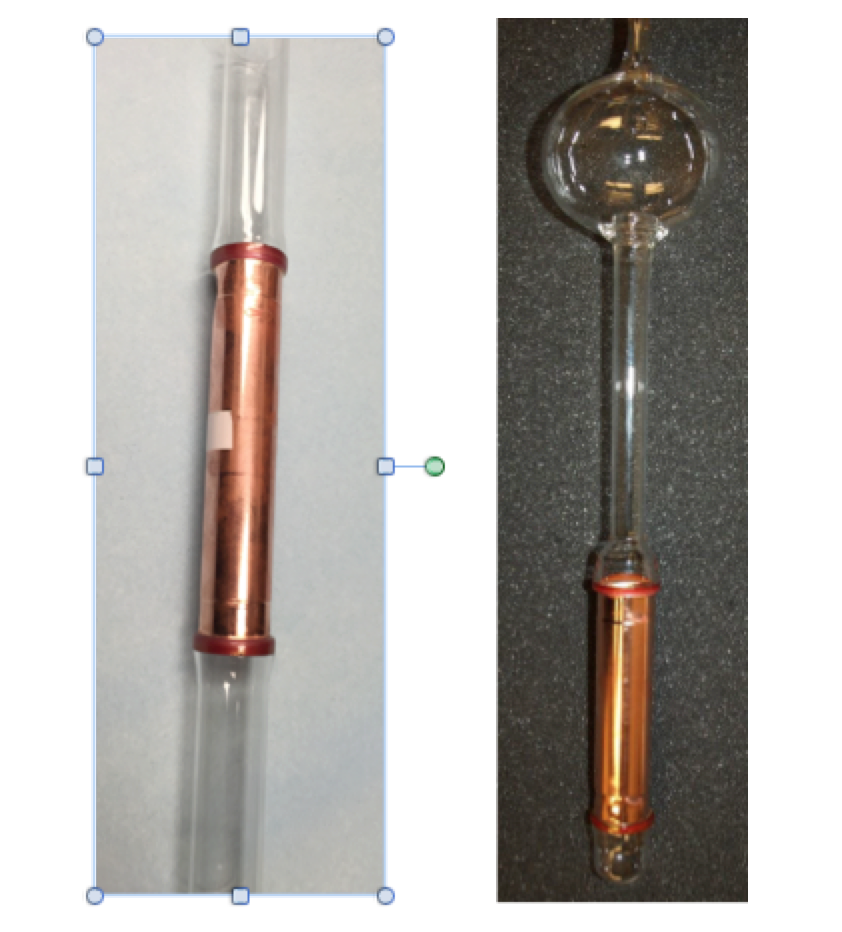
\includegraphics{metal_tube.png}}
	\caption{{Shown is a glass-to-metal-to-glass seal. The metal tube is 5'' long by 1'' outer diameter. The glass is wetted onto the knife-edge of copper on both ends.}}
	\label{metal_tube}
\end{figure}

The copper used in our tests is OFHC (oxygen-free high thermal conductivity) copper. In the earlier stage of our tests, OFHC copper was attached to the Pyrex glass, in which case a direct connection could be made. For the later tests where we were moving closer to the final goal of using metal end windows with the impermeable aluminosilicate glass GE180, a transition glass between OFHC copper and GE180 had to be used. The coefficient of expansion for GE180 glass is not compatible for making a direct seal with OFHC copper, thus Corning 7052 Kovar sealing glass was used as the transition. The two materials connected by a seal should have similar coefficients of expansion, the 7052 Kovar sealing glass serves as an intermediate material to bridge the gap between OFHC copper and GE180. The other type of metal used in our glass-to-metal seals was titanium, for which only Pyrex was used.

\subsection{Mechanical and Electropolishing}

The mechanical polishing is done by our machine shop in the department. A wire brush attached to a lathe was placed inside the tube while the lathe spun. This first-step polishing produced a relatively smooth surface in preparation for the following electropolishing process.

After the tubes were mechanically polished by the machine shop, they were sent to Able for electropolishing. The tube serves as the cathode, whihc is immersed in a temperature-controlled bath of electrolyte and connected to the positive terminal of a DC power supply, while the cathode is the attached to the negative terminal. During electropolishing, the polarized film is subjected to combined effects of gassing (oxygen) that occurs with electrochemical metal removal, saturation of the surface with dissolved metal and the agitation and temperature of the electrolyte. Metal on the surface is oxidized and dissolved in the electrolyte, the microscopic high points on the surface dissolve faster than the rate of attack on the rest parts of the surface, which provides a smoothing effect. As a result, the electropolishing process removes a thin layer of metal (about 20 $\mu m$ for our tubes), leaving a microscopically smooth and featureless surface. By contrast, even a fine mechanically polished surface will still show smears and other directionally oriented patterns or effects\cite{Electropolishing}. Fig.~\ref{Electropolishing} shows a diagram of the polishing process and its smoothing effect.

\begin{figure}[t!]
	\centering
	\resizebox{0.91\textwidth}{!}{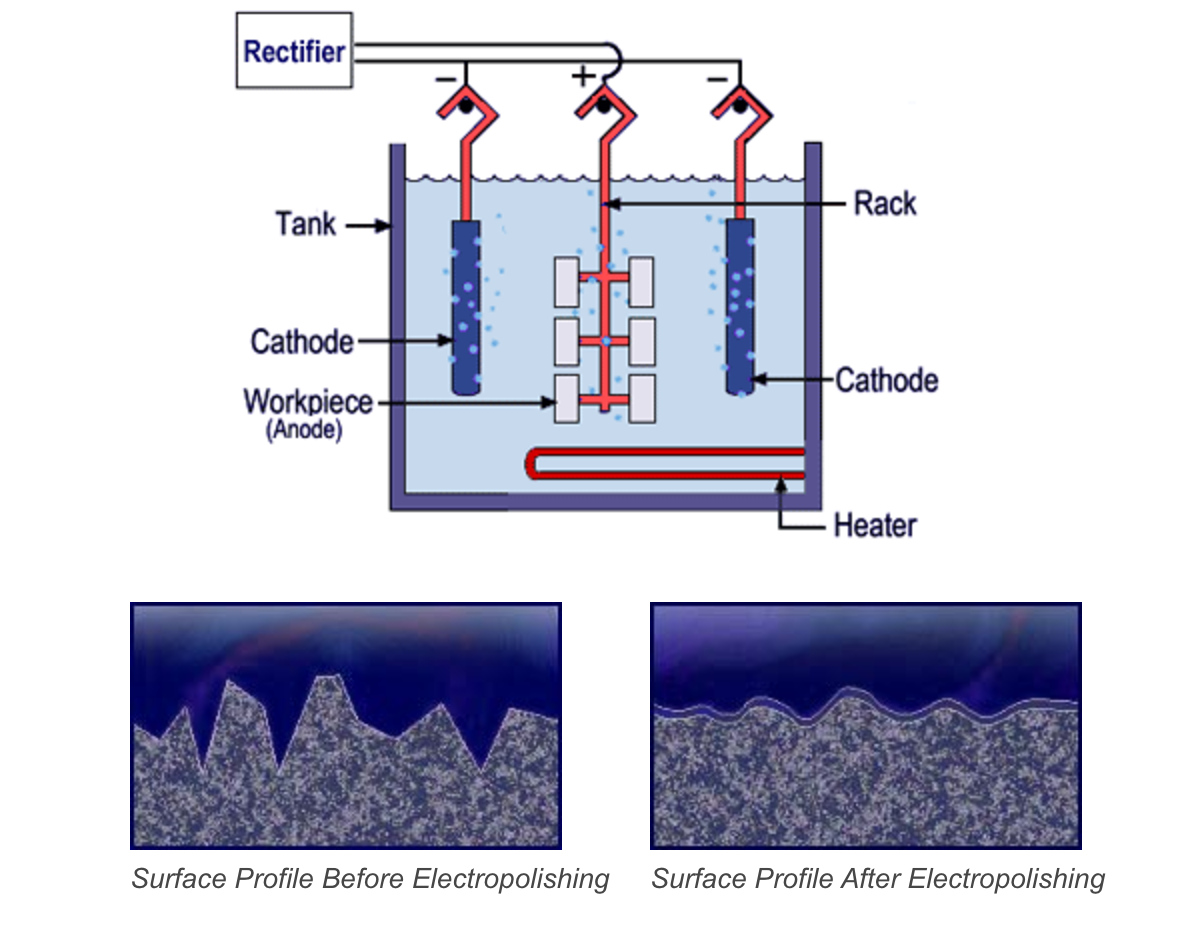
\includegraphics{Electropolishing.png}}
	\caption{{Electropolishing~\cite{Electropolishing}}}
	\label{Electropolishing}
\end{figure}

\subsection{Electroplating}

As stated earlier, because of the good lifetime reported by Deninger~\emph{et al.}, gold was plated on the inner surface of the OFHC copper and titanium tubes. Epner Technology Inc. handled the electroplating for us. Electroplating is the reverse process of electropolishing. When electric current passes through the electrolyte, the electrolyte splits up and some of the desired metal atoms it contains are deposited in a thin layer on top of the electrodes. Nickel an chromium are two common undercoatings used for electroplating, however, they are both ferromagnetic and can't be used for us as they would introduce additional spin relaxations. As a result, Epner used a copper strike to improve the durability of gold coating. A 5 $\mu m$ layer of gold was subsequently electroplated on the inner surface of the tubes. Fig.\ref{gold_coating} shows a comparison of a OFHC copper tube with gold-coating and a tube without any coating. 

\begin{figure}[t!]
	\centering
	\resizebox{0.91\textwidth}{!}{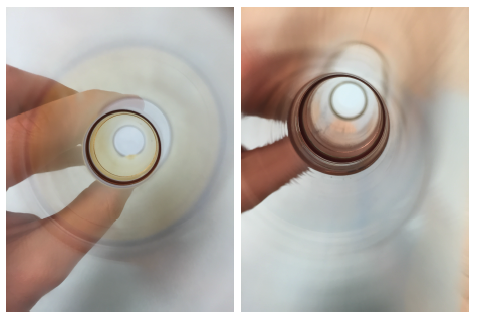
\includegraphics{gold_coating.png}}
	\caption{{Shown left is the inner surface of a gold coated OFHC copper tube. Shown right is a OFHC copper tube without coating.}}
	\label{gold_coating}
\end{figure}

\subsection{Final Assembly of the Cell}

After the tubes were coated and shipped back to us and leak checked one more time, they were cleaned with our ultrasonic cleaner. Fig.~\ref{ultrasonic_cleaner} shows the setup of the cleaning process. We cleaned the impurities on the surfaces of the tubes with ethanol, deionized water and methanol for thirty minutes each. As shown in the figure, a beaker containing the chemical solution and the tubes were placed in water bath inside the ultrasonic cleaner. Because of the dimensions of the cleaner and the beaker, we cleaned one end of the tubes first then flipped them to clean the other end before switching solution.

\begin{figure}[H]
	\centering
	\resizebox{0.4\textwidth}{!}{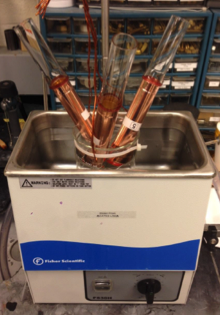
\includegraphics{ultrasonic_cleaner.png}}
	\caption{{Ultrasonic cleaner with 3 tubes being cleaned.}}
	\label{ultrasonic_cleaner}
\end{figure}

The test tubes were then shipped to our glassblower Mike Souza at Princeton University. All glass was reblown to the right size to reduce micro-fissures which would lead to high relaxation rate. The test tube was spliced with transfer tube and a pumping chamber. A string (see Fig.~\ref{string}) which would be used for cell filling was also made at Pricenton. Traditionally, a pure glass cell would be placed entirely in a oven for annealing. A cell made with GE180 would go through a five-minute ramping time to 780$^{\circ}C$, stay at 780$^{\circ}C$ for five minutes and slowly cool down to room temperature for at least 5 hours~\cite{DanThesis}. A Pyrex cool would be annealed in the exact same way except the highest temperature would be 565$^{\circ}C$. However, most our test cells could not have been annealed in the same way because of the glass-to-metal seal. Had we expose the seal to high temperature for long period of time, gold atoms might have migrated into the metal substrate and the seal might even break. Thus the metal tubes were attached to the rest of the glass parts after the pure glass parts were annealed. The finished cells together with glass strings were shipped to us.

\begin{figure}[t!]
	\centering
	\resizebox{0.91\textwidth}{!}{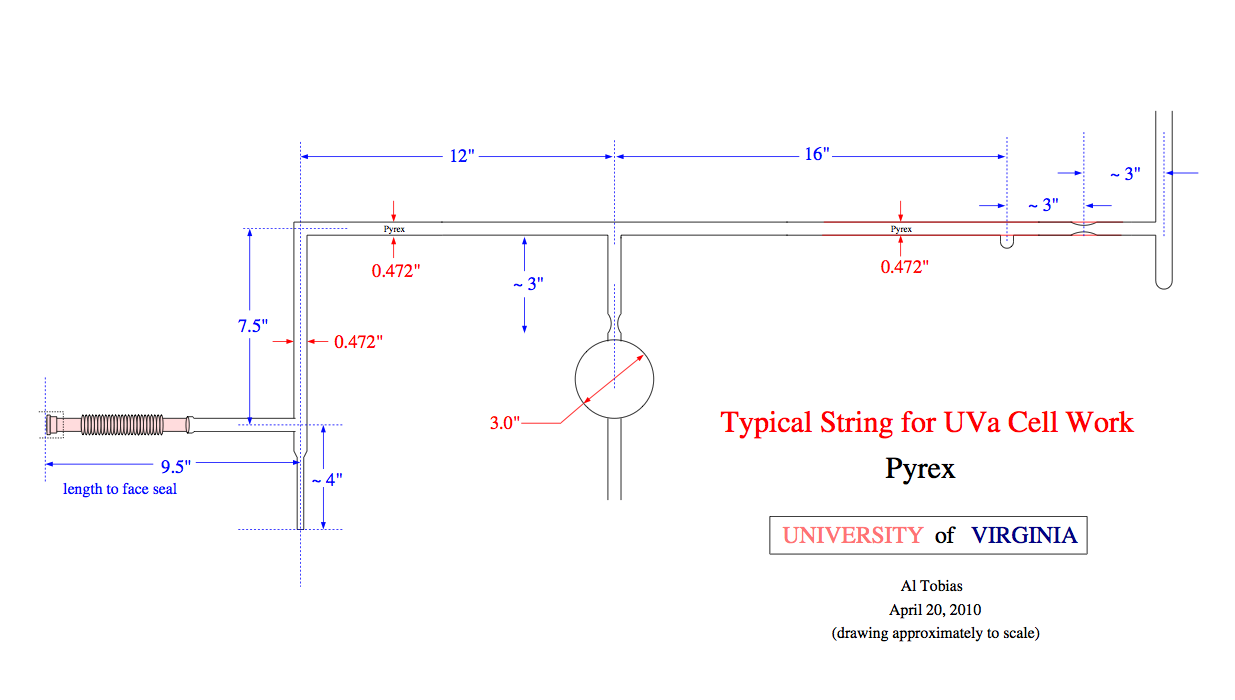
\includegraphics{string.png}}
	\caption{{Shown is the design of a typical string for our test cells.}}
	\label{string}
\end{figure}

\subsection{Cell Fill Procedure}

The details of cell fill was described thoroughly by Matyas~\cite{DanThesis}, I will briefly cover the process for the sake of completeness.

\subsubsection{Cell Fill Preparation}

Although the actual cell fill work only took less than a day, the preparation that led to the fill usually took 10-15 days. The string, cell and the retort (see Fig.\ref{}) were spliced together and attached to our homemade gas system through the bellows. a pre-scored ampoule of alkali metal was dropped from the top the of the retort.  Fig.~\ref{cell_gas_system} is a diagram of the string, cell and retort all connected together. 

\begin{figure}[t!]
	\centering
	\resizebox{0.91\textwidth}{!}{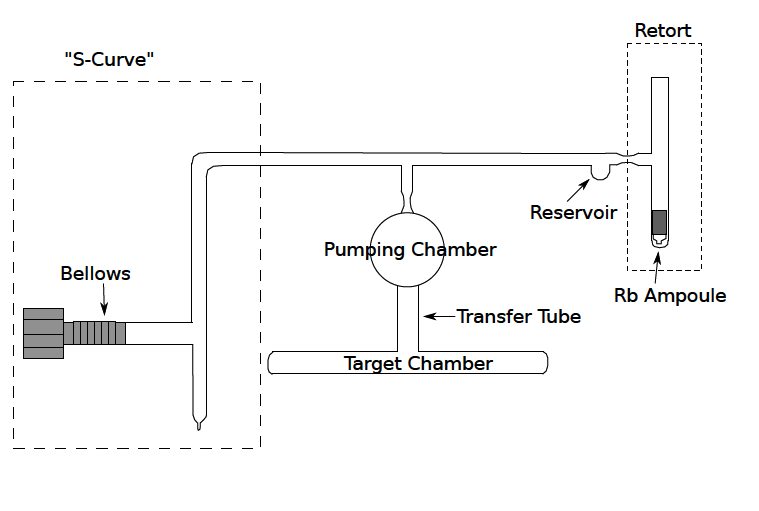
\includegraphics{cell_gas_system.png}}
	\caption{{A diagram of a Pyrex string with a cell and a retort attached while connected to the gas system through the bellows. Adapted from Matyas~\cite{DanThesis}.}}
	\label{cell_gas_system}
\end{figure}

The entire system was first rough-pumped down with a mechanical pump, and then kept being pumped by a diffusion pump to even lower vacuum. After the system was pumped for a few days and alkali metal was added in the system, we would keep pumping the system with the diffusion pump for roughly a week. To prevent the hot oil in the diffusion pump from going up into the gas system and the cell, a cold trap above the diffusion pump was filled every day with liquid nitrogen. "Flamebakes" were also performed 2-3 times a day during the one-week pumping period. A methane-oxygen torch was used to gently bake on the glass parts in the flamebakes. The bake should start from the retort which the farthest away from the diffusion pump, and move slowly towards the bellows, so the impurities chased off the inner surfaces can be "swept" towards the pump leaving as few impurities behind as possible. The alkali metal was typically melted on the second or third flamebake and should be melted during each of the remaining flamebakes. On the day before the fill, alkali metal was melted and chased into the pumping chamber.

\subsubsection{Cell Fill}

The first thing on the fill day was to make sure pump all portions of the gas system to vacuum and selectively back fill some parts with appropriate gases (either N$_2$ or $^{3}$He) to minimize outgassing. The gas filled into the cell should always be cleaned during the path to the cell. Earlier test cells were filled with the noble gas purifier while the later cells were done with a homemade cold trap.

The homemade cold trap consisted of a copper tubing placed inside box-shaped Dewar. The Dewar was filled with liquid nitrogen when filling N$_2$ and liquid helium when filling $^{3}$He, so impurities in the gas were frozen in the copper tubing. Temperature inside the dewar was monitored with two silicon diodes to determine whether copper tubing was fully submerge in the cold liquid.

The volume of the cell was also determined during the fill process. A Baratron pressure gauge was used to measure a calibrated volume (CV) of 992.9 cc. 300 Torr of gas was filled into the calibrated volume, then the valve on CV was closed and any gas outside of CV was pumped away. Next the gas kept in CV was let out into the fill gap between CV and the string while monitoring pressure with the Baratron gauge, thus the volume of the cell could be calculated with ideal gas law.

Around 70 Torr of nitrogen was put into the cell before filling $^{3}$He. To prevent nitrogen from escaping the cell while filling $^{3}$He, the string valve was kept closed until $^{3}$He pressure in fill gap rose well above 70 Torr. A total gas pressure of just under 760 Torr (1 atm) was reached. This target pressure was chosen because when the connection between the cell and the string was melted, the atmospheric pressure would collapse it and seal the cell for us. All cells except Kappa1 contained pure rubidium, while Kappa1 was contained 5:1 alkali mixture of potassium to rubidium.

\section{Experimental Procedure}

All cells incorporated metal were tested with Pulse NMR as it is only affects a small region of the cell and minimizes influences from eddy current in the metal tubes. Kappa1 was a simple spheric and pure GE180 cell, which was built to rule out the possibility that the melt of GE180 our cells had been made of was bad. Because of its lack of metal and lack of convenient places to wrap pickup coils on, Adiabatic Fast Passage was used to test Kappa1. Both PNMR and AFP were discussed in a general way in chapter 3, I will add on to the discussions with more specific experimental setups for this study.

\subsection{Pickup Coils}

In a AFP measurement, pickup coils are placed next to the side windows of the oven. However, the same setup proved to be more difficult for us to receive high-quality PNMR signals. To still keep the pickup coils outside of the oven, we manually wrap a solenoid coil on the transfer tube of test cells where it is approximately 2'' below the bottom of the oven. These coils were made with 40-50 turns of AWG 20 copper wire. Because of the off-center positions of the pickup coils, inhomogeneities were significant enough to affect FID signals, gradient coils were used to cancel the inhomogeneities.

\subsection{Gradient Coils}

Inhomogeneities were canceled to the best we could empirically with three sets of gradient coils. Each set of gradients coils consists of two oppositely wound coils separated by a distance $d$, this particular type of coils are referred to as "Maxwell coils". The setup is very similar to that of Helmholtz coils, except the opposite direction of currents and the larger optimum separation $d=R$, where $R$ is the radius of the coils. The opposite direction is to cancel out the magnetic field at the center, and the optimum separation makes the first four leading terms in the Taylor expansion zero\cite{Callaghan}. Fig.\ref{gradient_coils} shows the coil orientations. The z axis is defined to be aligned with the direction of the holding field while x and y axes are in the transverse plane. The direction of coil axis is then defined by the angle $\theta$ and $\phi$, where $\theta$ is with respect to the z axis and $\phi$ is the azimuthal angle in the x-y plane.

\begin{figure}[t!]
	\centering
	\resizebox{0.91\textwidth}{!}{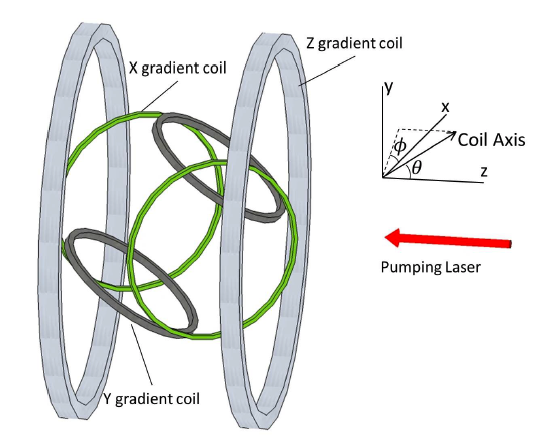
\includegraphics{gradient_coils.png}}
	\caption{{Diagram of the coils. Adopted from Zheng~\cite{YuanThesis}.}}
	\label{gradient_coils}
\end{figure}

The magnetic field at the center is given by\cite{PhysRevA.37.2877}

\begin{equation}\label{gradient}
\begin{split}
\nabla\boldsymbol{B}(\theta, \phi)
&=\begin{bmatrix}
\partial B_x/\partial x & \partial B_y/\partial x & \partial B_z/\partial x \\
\partial B_x/\partial y & \partial B_y/\partial y & \partial B_z/\partial y \\
\partial B_x/\partial z & \partial B_y/\partial z & \partial B_z/\partial z
\end{bmatrix}\\
&=3\kappa I
\begin{bmatrix}
sin^2\theta cos^2\phi-\frac{1}{3} & sin^2\theta sin\phi cos\phi & sin\theta cos\theta cos\phi \\
sin^2\theta sin\phi cos\phi & sin^2\theta sin^2\phi-\frac{1}{3} & sin\theta cos\theta sin\phi \\
sin\theta cos\theta cos\phi & sin\theta cos\theta sin\phi & cos^2\theta-\frac{1}{3}
\end{bmatrix}
\end{split}
\end{equation}
where the calibration constant $\kappa$ is:

\begin{equation}
\kappa = \frac{3\pi n R^2 d/2}{5(d^2/4+R^2)^{5/2}}G\,cm\,A^{-1}
\end{equation}

The most important terms in Eq.\ref{gradient} are those related to $B_z$: $\partial B_z/\partial x$, $\partial B_z/\partial y$ and $\partial B_z/\partial z$. The orientations of the gradient coils can be chosen such that each of the three sets of coils controls one of the aforementioned terms. This "magic angle" $\theta_m$ is given by

\begin{equation}
\theta_m = cos^{-1}1/\sqrt{3}=54.7^{\circ}
\end{equation}

For $\theta=\theta_m$ and $\phi=0$ the gradient tensor is

\begin{equation}
\nabla\boldsymbol{B}(\theta_m, 0)=\kappa I
\begin{bmatrix}
1 & 0 & \sqrt{2}\\
0 & -1 & 0 \\
\sqrt{2} & 0 & 0
\end{bmatrix}
\end{equation}

For $\theta=\theta_m$ and $\phi=\pi/2$ we have

\begin{equation}
\nabla\boldsymbol{B}(\theta_m, 0)=\kappa I
\begin{bmatrix}
-1 & 0 & 0\\
0 & 1 & \sqrt{2}\\
0 & \sqrt{2} & 0
\end{bmatrix}
\end{equation}

Finally, for the z gradient coil we have

\begin{equation}
\nabla\boldsymbol{B}(\theta_m, 0)=\kappa I
\begin{bmatrix}
-1 & 0 & 0\\
0 & -1 & 0\\
0 & 0 & 2
\end{bmatrix}
\end{equation}

Our gradient coils were built by Zheng~\cite{YuanThesis}. The separations were do not follow the optimum condition $d=\sqrt{3}R$ due to spatial limitations. The dimensions of the gradient coils are shown in Table~\ref{gradient_coils_table}.

\begin{center}
	\begin{tabular}{ | c | c| c| c | }
		\hline
		& turns & radius & separation \\ \hline
		x & 42 & 33 cm & 64 cm \\ \hline 
		y & 100 & 28 cm & 56 cm \\ \hline
		z & 8 & 66 cm & 66 cm \\
		\hline
	\end{tabular}
\end{center}\label{gradient_coils_table}

\subsection{Laser Setup}







